\chapter{Methodology}

\section{Observations used for evaluation of climate models}
A global comparison of simulated present day climate with observations requires a global set of observations with a significantly long record. A number of relevant climatologies of cloud properties from satellite observations has been developed for this purpose \citep{stubenrauch_et_al_2009}. These climatologies use a variety of instruments, each with their own strengths and weaknesses. This study focuses on climatologies from passive remote sensing instruments for which instrument simulators have been developed and included in COSP. These include the GEWEX ISCCP \citep{rossow_and_schiffer_1999}, MISR \citep{diner_et_al_1998,diner_et_al_2002,diner_et_al_2005}, and MODIS \citep{king_et_al_2003}. The climatologies from these instruments have distinct differences owing to differences in the retrieval process and, in many ways, offer both supplementary and complementary views of clouds in the atmosphere \citep{marchand_et_al_2010,pincus_et_al_2011}. The climatologies used in this study were assembled specifically for comparison with climate models using instrument simulators, and all are available at \url{http://climserv.ipsl.polytechnique.fr/fr/cfmip-observations.html}. These datasets are described in detail in the references \citep{marchand_et_al_2010,pincus_et_al_2011}, and the essential properties of each are briefly summarized below.

ISCCP provides the longest record by far of any of the climatologies used here (26 years, as opposed to the nine year records of MISR and MODIS). ISCCP collects observations from a suite of geostationary and polar orbiting satellites and uses this data to flag cloudy pixels and estimate cloud top pressure $p_c$ and optical thickness $\tau$ \citep{rossow_and_schiffer_1999}. Retrieval of cloud top pressure is a multi-step process. First, cloud top temperature is estimated from the observed infrared brightness temperature. Cloud top pressure is then inferred from the cloud top temperature using an atmospheric profile obtained from sounding instruments to relate temperature to pressure. If cloud top pressure cannot be determined, a cloud top pressure is assigned that is just above the tropopause. Cloud optical thickness is inferred from the observed visible wavelength radiances using pre-computed tables based on one-dimensional radiative transfer. Clouds are assumed to be single layered with a constant particle size distribution that is selected based on the observed infrared brightness temperature.

The ISCCP climatology used in this study is derived from the ISCCP D1 product (\url{http://isccp.giss.nasa.gov}) and similar to the ISCCP D2 product. The D1 data is saved on an equal-area grid with 3-hourly resolution. This data is interpolated to an equal-angle grid and averaged over all daytime values in a month at once. The climatology includes estimates of mean cloud albedo, cloud top pressure, and cloud top temperature, all weighted by the total cloud fraction at each time. The climatology includes day-time only data over the period July 1983 to June 2008. Of primary importance to this study is the full resolution joint histogram of cloudiness with cloud top pressure and cloud optical thickness. Because each cloudy pixel is assigned only one estimate of cloud top pressure and cloud optical thickness, summing all values in this histogram produces the total cloud amount. Likewise, low-topped cloud amount is estimated by summing all histogram bins with $p_c>680~\text{hPa}$, mid-topped cloud amount is estimated by summing all histogram bins with $680>p_c>440~\text{hPa}$, and high-topped cloud amount is estimated by summing all histogram bins with $p_c<440~\text{hPa}$. Optically thick cloud amount is estimated by summing all histogram bins with $\tau>23.0$.

The MODIS instrument is a 36-channel scanning radiometer \citep{king_et_al_2003}. MODIS instruments operate on both the Terra and Aqua satellites, and data products from either are available, as well as a product that averages the two separate instruments. For clouds with cloud top pressures less than about $700 ~\text{hPa}$, a $\text{CO}_2$ slicing technique \citep{menzel_et_al_1983} is used to estimate cloud top pressure. This technique fails for clouds with cloud top pressures above this threshold, so cloud top pressure for low-topped clouds is inferred from the MODIS retrieved $11 ~\mu\text{m}$ brightness temperature using an independently observed atmospheric temperature profile in a manner similar to the ISCCP cloud top pressure retrieval. Similarly to the ISCCP cloud optical thickness retrieval, the MODIS cloud optical thickness retrieval uses pre-computed tables based on one-dimensional radiative transfer to relate observed radiance to optical thickness. However, the multiple channels of the MODIS instrument allow this to be done for multiple wavelength bands. The MODIS retrieval of optical thickness uses calculations in two different bands to estimate the cloud optical thickness and effective particle size simultaneously based on the thermodynamic phase determined from a variety of tests in different wavelength bands.

The MODIS climatology used in this study uses a combination of day-time only data from MODIS instruments aboard both the Terra and Aqua platforms over the time period July 2002 to July 2010. This climatology includes a number of cloud property observations, including separate total cloud amount estimates for liquid, ice, and all clouds; estimates of low, mid, and high-topped clouds; column integrated liquid and ice water paths; mean effective particle sizes for both liquid and ice phase clouds; mean cloud top pressure; linear mean optical thickness ($\overline{\tau}$) for liquid, ice, and all clouds; and base-10 logarithm weighted optical thickness ($10^{\overline{\log{\tau}}}$) for liquid, ice, and all clouds. All retrieved cloud properties are weighted by the appropriate cloud amount (liquid or ice cloud amount in the case of liquid and ice cloud properties). Of primary interest to this study, the distribution of cloudiness with cloud top pressure and optical thickness are included in a joint histogram field using the same bins as in the ISCCP climatology. Estimates of optically thick, total, low, mid, and high-topped cloudiness are computed in the same way from the MODIS climatology as from the ISCCP climatology.

The MISR instrument is a radiometer aboard the Terra satellite platform, consisting of nine separate viewing cameras, each collecting data at a different view angle \citep{diner_et_al_1998,diner_et_al_2002,diner_et_al_2005}. These nine successive views of the earth and atmosphere allow MISR to use a stereo-imaging technique to infer cloud top height $z_c$. Cloud top height determined by this method is independent of the actual values of the observed radiances \citep{moroney_et_al_2002,muller_et_al_2002}. Similarly to ISCCP, the MISR retrieval of cloud optical thickness is inferred from the observed visible wavelength radiances. The optical thickness retrieval assumes clouds are single-layered with a fixed effective particle size. Contrary to the ISCCP and MODIS retrievals, the MISR optical thickness retrieval is only performed over ice-free oceans. Joint histograms of cloudiness with cloud top height and optical thickness are produced, but the bins used in these histograms differ somewhat from those produced by ISCCP and MODIS because MISR retrieves cloud top height, as opposed to ISCCP and MODIS that retrieve cloud top pressure. The MISR histogram includes more bins in the vertical than ISCCP or MODIS (16 cloud top height bins for MISR as opposed to seven cloud top pressure bins for ISCCP and MODIS). MISR also has ``no retrieval'' bins for both the cloud top height and optical thickness for cases in which a pixel is flagged as cloudy by the radiometric cloud mask, but either the cloud top height or optical thickness retrieval fails.

The MISR climatology used in this study is from the MISR L3 CTH-OD V5 dataset, and includes day-time, ice-free ocean-only data over the period March 2000 to November 2009. Monthly, seasonal, and annual climatologies are computed over the entire record for use in this study. The MISR dataset contains only the joint histogram product, from which estimates of total, low, mid, or high-topped cloud amount can be computed over a choice of optical thickness ranges similarly to estimates of cloudiness computed from the ISCCP and MODIS joint histogram products. Total cloudiness is computed by summing over all cloud top height bins (including the ``no retrieval'' bin). Low-topped cloud is computed by summing over cloud top height bins with $0.0<z_c<3.0~\text{km}$, mid-topped by summing over cloud top height bins with $3.0<z_c<7.0~\text{km}$, and high-topped by summing over cloud top height bins with $z_c>7.0~\text{km}$. These thresholds roughly correspond to those used in the calculation of cloud types from the ISCCP and MODIS joint histograms based on cloud top pressure. For all cloud types, the summation is restricted to optical thickness bins for which $\tau>0.3$. This represents the limit of the distribution for which the three passive sensors considered here can reliably detect cloud, although to improve agreement across the different sensors there are arguments to use a higher threshold \citep{marchand_et_al_2010,pincus_et_al_2011}. Nonetheless, the $\tau>0.3$ threshold is used here for consistency with prior studies \citep[e.g.,][]{marchand_and_ackerman_2010}.

Each of these passive instruments has their own strengths and weaknesses, owing to the differences in the cloud property retrievals of the three. These strengths and weaknesses are explored in detail in \cite{marchand_et_al_2010} and \cite{pincus_et_al_2011}, but a brief discussion is provided here of those of particular importance to this study.

As noted in both \cite{marchand_et_al_2010} and \cite{pincus_et_al_2011}, there is a somewhat large difference between the number of pixels that the MODIS cloud mask flags as cloudy and those for which cloud property retrievals are performed. This is due to a more selective criteria for determining suitable pixels for which to perform retrievals. Part of this criteria is a restriction to only perform optical thickness and particle size retrievals for pixels that are not deemed to exist at the edge of a cloud boundary. This leads to two distinct cloud fractions retrieved from MODIS: that retrieved from the cloud mask, and that for which optical thickness and particle size retrievals are performed, which is referred to as the ``retrieval cloud fraction''. The process of removing cloud boundary pixels is referred to as ``clear-sky restoral'' and can cause large discrepancies between the two different estimates of cloud fraction especially in regions of broken cloud, such as in the subtropical trade cumulus regions. In these regions a substantial number of pixels are removed from the retrieval cloud fraction, causing the retrieval cloud fraction to be biased low compared with cloud fraction estimates from ISCCP and MISR \citep{marchand_et_al_2010,pincus_et_al_2011}. Estimates of total cloudiness from ISCCP, MISR, and MODIS are shown in Figure \ref{clt_retrievals_map}. Both estimates of cloud fraction from MODIS are shown.
\begin{figure}
    \centering
    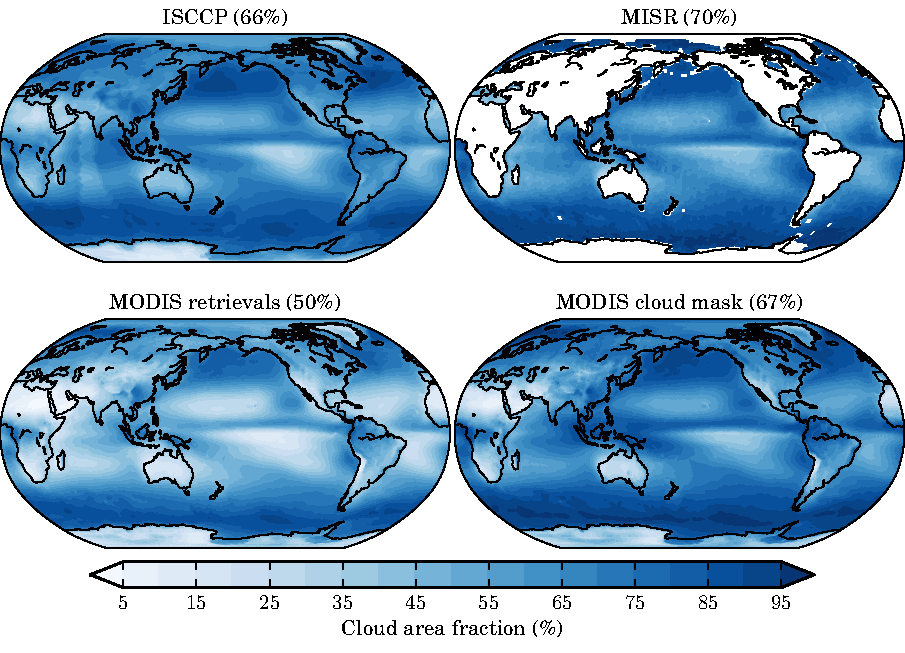
\includegraphics{../graphics/clt_retrievals_map.pdf}
    \caption[Estimates of total cloudiness from ISCCP, MISR, and MODIS observations.]{Estimates of total cloudiness from ISCCP, MISR, and MODIS observations. The MISR cloud amount estimate only includes clouds with optical thickness $\tau>0.3$. For MODIS, both the fraction of clouds for which optical thickness and particle size retrievals are successful are shown alongside the fraction of clouds flagged as cloudy by the cloud mask. The MODIS retrieval cloud amount only includes clouds with optical thickness $\tau>0.3$. The area-weighted global mean is indicated in the title of each plot.}
    \label{clt_retrievals_map}
\end{figure}

Since cloud top pressure retrievals are performed on all pixels identified as cloudy by the cloud mask, estimates of low, mid, and high-topped cloud that are in better agreement with those calculated from the ISCCP and MISR joint histograms can be derived from the cloud top pressure histogram before clear-sky restoral than those calculated from the full joint histogram of cloudiness with cloud top pressure and optical thickness. Comparisons between MODIS-simulated and MODIS-observed low, mid, and high-topped cloud in this study will use the estimation of these cloud amounts from MODIS calculated from the cloud top pressure histogram before clear-sky restoral. This is somewhat of a trade-off, as this practice is inconsistent with the cut-off of clouds below the optical thickness threshold used for the ISCCP and MISR comparisons. However, the simulators have no way of accounting for the low population of clouds in the MODIS retrieval due to clear-sky restoral, and comparisons with the retrieval cloud amount would therefore be misleading. The retrieval cloud amount will be used in analysis with the full cloud top pressure and optical thickness joint histograms, and the relatively low population of clouds in the retrieval cloud amount should be kept in mind when considering these histograms from MODIS compared with ISCCP and MISR.

The MODIS clear-sky restoral process also affects the optical thickness distribution. \cite{pincus_et_al_2011} show that MODIS retrieved clouds are often more optically thick than those retrieved by ISCCP, the implication being that the majority of pixels removed by the clear-sky restoral process are optically thin, and cloud fractions for optically thicker clouds should be expected to agree much better between the three instruments.

The dependence of the retrieved cloud top pressure on observed atmospheric profiles makes ISCCP and MODIS observations of cloud top pressure susceptible to errors in these profiles. This frequently occurs in cases associated with strong temperature inversions such as in stratocumulus in regions of large-scale sub-tropical subsidence \citep{marchand_et_al_2010}. In such cases the ISCCP and MODIS retrieved cloud top pressure is often biased low. MISR does not suffer from this limitation, and cloud top heights retrieved by MISR in these situations can be considered to be more reliable than cloud top pressures retrieved from ISCCP and MODIS \citep{marchand_et_al_2010}.

As described in \cite{marchand_et_al_2010}, ISCCP, MISR, and MODIS can differ substantially in their estimates of cloud top height for pixels that contain optically thin cirrus over a thicker cloud layer. The stereo-imaging technique used by MISR relies on comparing distinct cloud features with surface features in multiple views to infer the height of cloud tops using parallax. In cases where the upper cloud layer is sufficiently optically thin, MISR preferentially identifies features of the lower cloud layer and infers the height of the lower level cloud top instead of the optically thin upper level cloud. This occurs frequently for cases in which the optical thickness of the upper cloud layer is less than $\tau = 5$ \citep{marchand_et_al_2007}. The tendency for MISR to effectively ``see'' through optically thin cirrus causes MISR estimates low-topped cloud amounts to be higher (and estimates of high-topped cloud amount to be lower) compared to those estimated from ISCCP or MODIS in regions in which optically thin cirrus frequently overlap lower cloud layers.

The ISCCP retrieval of cloud top pressure assumes that clouds radiate as black bodies to infer a cloud top temperature from measured radiances. For clouds that are sufficiently thin the thermal emission signature can differ substantially from that of a black body, and thermal emission from the surface or underlying cloud layers can increase the observed brightness temperature. In these cases the ISCCP retrieval of cloud top pressure essentially responds to the radiative mean cloud top pressure between the two layers, and retrieved cloud top pressure can be expected to be higher than the actual cloud top pressure of the cloud layer. This can cause ISCCP to bias high-topped clouds into mid-levels. $\text{CO}_2$ slicing techniques such as that used by MODIS have been shown to also be susceptible to retrieving a weighted mean of the two cloud layers when optically thin cirrus overlaps a lower cloud layer \citep[e.g.,][]{baum_and_wielicki_1994}, although \cite{marchand_et_al_2010} suggest that the effect is smaller for the MODIS $\text{CO}_2$ slicing technique than for the ISCCP brightness temperature technique.

This study makes extensive use of joint histograms of cloudiness as a function of both cloud top height (or pressure) and cloud optical thickness. Comparisons of cloudiness with cloud top pressure can be obscured by fact that MISR measures cloud top height in units of height while ISCCP and MODIS measure cloud top pressure. To make these comparisons more transparent, the bins of each histogram can be collected into a coarser set of nine histogram bins. Clouds can broadly be classified as low-topped ($p_c>680~\text{hPa}$, $0.0<z_c<3.0~\text{km}$), mid-topped ($680>p_c>440~\text{hPa}$, $3.0<z_c<7.0~\text{km}$), or high-topped ($p_c<440~\text{hPa}$, $z_c>7.0~\text{km}$), and optically thin ($\tau<3.4$), optically intermediate ($3.4<\tau<23.0$), and optically thick ($\tau>23.0$). These classifications are consistent with previous studies using the ISCCP observations and the ISCCP simulator \cite[e.g.,][]{zhang_et_al_2005}. 

Evaluation of model cloud properties is done in the context of the impact on the radiative budget. Radiative quantities from models are compared with those from version 2.5 of the Clouds and the Earth's Radiant Energy System Energy Balanced and Filled (CERES-EBAF) dataset \citep{loeb_et_al_2009}. The climatology used here covers a 10 year period from March 2000 to February 2010.

\section{Overview of models for evaluation}
Simulations are performed with four different models in this study. First, simulations of present-day clouds are evaluated from two models that participated in the World Climate Research Programme (WCRP) CMIP3 \citep{meehl_et_al_2007}: The National Center for Atmospheric Research (NCAR) Community Atmosphere Model version 3 \citep[CAM3;][]{cam3_description}, and the Geophysical Fluid Dynamics Laboratory (GFDL) Atmosphere-only Model version 2 \citep[AM2;][]{am2_evaluation}. These models were chosen for their widespread use and known differing responses to climate change scenarios, as will be explored in following chapters (see, for example, Figure 1 of \cite{stephens_2005}, although an earlier version of CAM is used in that study). These models differ in both their dynamics and their physics parameterizations, although no attempt is made here to disentangle the effects of each of these independently. The default dynamical core used in AM2 is a finite volume core, while CAM3 uses an Eulerian spectral transform core. A finite volume dynamical core is also supported in CAM3, and simulations will be shown using both dynamical cores in Chapter \ref{camamip}. Both AM2 and CAM3 treat non-convective cloud condensate using a prognostic scheme, with separate evolution equations for liquid and ice condensate. Cloud microphysics in AM2 are parameterized according to \cite{rotstayn_1997}, while CAM3 implements the scheme described in \cite{rasch_and_kristjansson_1998} and \cite{zhang_et_al_2003}. For cloud fraction, AM2 implements the prognostic scheme described by \cite{tiedtke_1993}, while CAM3 implements a diagnostic cloud scheme that generalizes and modifies the scheme described by \cite{slingo_1989}. Cloud overlap also differs between AM2 and CAM3, with AM2 implementing random overlap and CAM3 implementing maximum-random overlap. \cite{am2_evaluation} point out that the assumption of random overlap in AM2 is acceptable in the upper troposphere due to coarse model vertical resolution, but that the assumption is poor for clouds in the lower troposphere. The configuration of these models is briefly summarized in table \ref{models}, and more details are described in the references.
\begin{table}
    \centering
    \begin{tabular}{lccc}
        \hline
        Model & Institution & References                            & Configuration \\ \hline
        AM2     & GFDL                & \cite{am2_evaluation}     & Finite Volume $2^{\circ} ~\text{lat} \times 2.5^{\circ} ~\text{lon}$, $24$ levels \\ 
        CAM3    & NCAR                & \cite{cam3_description} & Eulerian T42 $2.8^{\circ} ~\text{lat} \times 2.8^{\circ} ~\text{lon}$, $26$ levels \\
        CAM4    & NCAR                & \cite{cam4_description} & Finite Volume $0.9^{\circ} ~\text{lat} \times 1.25^{\circ} ~\text{lon}$, $26$ levels \\
        CAM5    & NCAR                & \cite{cam5_description} & Finite Volume $0.9^{\circ} ~\text{lat} \times 1.25^{\circ} ~\text{lon}$, $30$ levels \\ \hline
    \end{tabular}
    \caption{Models used in this study.}
    \label{models}
\end{table}

Successive versions of the Community Atmosphere Model (CAM4 and CAM5) are also evaluated to assess the impact of changes made between versions on the simulated clouds. These models are also summarized in table \ref{models}, and full descriptions of each are contained in the references therein. Table \ref{models} shows that the default dynamical core in CAM4 and CAM5 has been changed since CAM3 from the Eulerian spectral transform core to a finite volume core. The resolution of simulations performed here with CAM4 and CAM5 is much higher than that used in the simulations with CAM3. The vertical resolution increases from CAM4 to CAM5 with the addition of model levels in the lower troposphere, nearly doubling the vertical resolution below $700~\text{hPa}$ \citep{medeiros_et_al_2011}.

Physics parameterizations in CAM4 are very similar to those in CAM3, with few changes. These changes include changes made to the deep convection \citep{neale_et_al_2008,richter_and_rasch_2008} and the addition of the so-called ``freeze-dry'' parameterization that acts to reduce the low cloud fraction in the absence of significant water vapor \citep{vavrus_and_waliser_2008}. In contrast, an almost completely new physics parameterization suite has been implemented in CAM5, with only the deep convection in CAM4 remaining common between the two models. The CAM5 implementation of COSP also includes radiatively active ``snow'', which in this context is simply large, precipitating ice crystals.

\section{Implementation of COSP in model diagnostics}
This study makes extensive use of the diagnostics provided by COSP. COSP can be implemented in-line with the model code, or can be run off-line if sufficient model output is available. For the evaluation of climate models on long time scales it makes much more sense to implement COSP in-line with the model radiation code. To run COSP off-line requires non-standard quantities to be output at very high temporal resolution in order to accumulate sufficient statistics and to reasonably depict the clouds, which vary on too short of time scales for statistics accumulated from monthly-mean fields to be of much use. It would require an extraordinary amount of disk space to store all of the model output required for anything longer than a very short model run. Running COSP in-line with the model gives the simulators access to the instantaneous model fields, allowing the simulators to be run at the high temporal resolution needed, but statistics can be accumulated and only the monthly means of these statistics need be saved. This greatly reduces the disk space requirements, and allows COSP diagnostics to be saved in the model output history files. Additionally, this approach takes advantage of the parallelization handled by the model, greatly reducing the computational time required to obtain usable diagnostics.

At the time this work began, neither NCAR nor GFDL had implemented COSP into their models, although the ISCCP simulator was included in the release versions of CAM3 and AM2. In order to evaluate CAM3 and AM2 using the instrument simulators, both models needed to be modified to run COSP in-line. This was mostly a matter of modifying the code used to call the ISCCP simulator. Only the passive sensor (ISCCP, MISR, MODIS) instrument simulators have been implemented. The active sensor simulators have not yet been implemented in these two models. The implementation of the passive sensors was tested by comparing output from the ISCCP simulator called from COSP with output from the ISCCP simulator called from the original model code without COSP. Results of this test showed only slight differences in the two implementations that were likely caused by the use of two different versions of the ISCCP simulator, which are known to produce slightly different results (description of simulator and differences is in the ISCCP simulator README file included in the COSP source code distribution). The implementation was also tested against off-line calculations with COSP using 3-hourly instantaneous model output fields, and found to produce nearly identical results. 

The work of implementing COSP in CAM4 and CAM5 has been accomplished largely by the efforts of Dr. Jennifer Kay at NCAR, among others, and is documented in \cite{kay_et_al_2011}. This is a full implementation of COSP, with both the passive and active sensor simulators. Inclusion of COSP in the release version of these models allows simulations to be performed using the production code for these models without modification.

\section{Strategies for evaluation and model intercomparison}
So-called ``Taylor diagrams'' \citep{taylor_2001} provide concise statistical summaries that lend themselves well to model intercomparisons \citep{gleckler_et_al_2008,pincus_et_al_2008}. These diagrams take advantage of the mathematical relationship of various statistical measures of comparison between two variables to represent them all on a single figure. An example is shown in Figure \ref{cldtot_obs_taylor}, comparing the annual cycle (monthly means over the entire record) of total cloudiness from ISCCP, MISR, and MODIS observations. The radial axis represents the ratio $\tilde{\sigma}$ of standard deviations between the test field $X$ and the reference field $Y$, where
\[
    \tilde{\sigma} = \frac{\sigma_X}{\sigma_Y}
        = \sqrt{\frac{\sum_{n=1}^N (X_n - \overline{X})^2}
            {\sum_{n=1}^N (Y_n - \overline{Y})^2}}.
\]
A ratio of unity implies that the test and reference field have identical variability. This is indicated on the diagram by a solid arc to denote the reference variance ratio of unity. The azimuthal axis represents the pattern correlation $R$ in space and time between the test field $X$ and reference field $Y$, where
\[
    R = \frac{{\rm cov}(X,Y)}{\sigma_X \sigma_Y}
      = \frac{\sum_{n=1}^N (X_n - \overline{X})(Y_n - \overline{Y})}{\sqrt{\sum_{n=1}^N (X_n - \overline{X})}\sqrt{\sum_{n-1}^N (Y_n - \overline{Y})}}.
\]
A correlation of unity implies that the two fields are perfectly correlated in both space and time. A point that intersects the reference curve and the horizontal axis would imply perfect agreement between the test and reference fields. The diameter of the circles concentric with each point on the diagram (measured using the same scale as that for the ratio of standard deviations) is equal to the absolute value of the relative bias $\tilde{E}$ in the test field compared with the reference field, where
\[
    \tilde{E} = \frac{\overline{X} - \overline{Y}}{\left|\overline{Y}\right|}.
\]

\begin{figure}
    \centering
    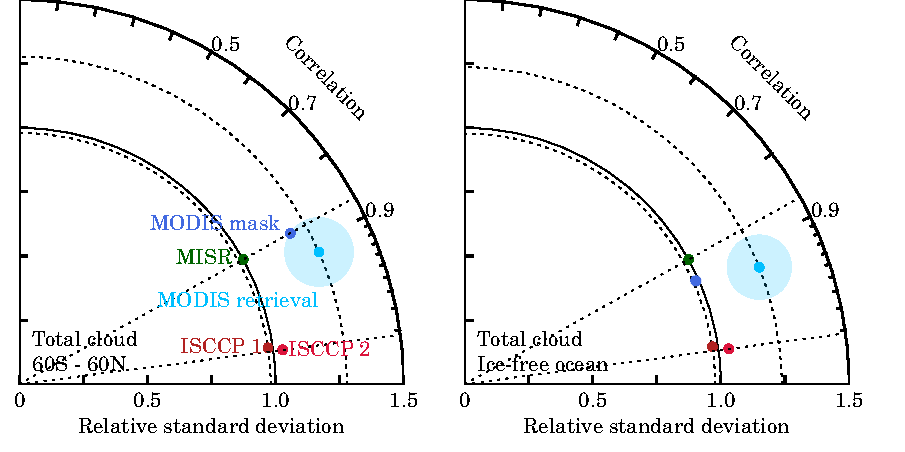
\includegraphics{../graphics/clt_retrievals_taylor.pdf} 
    \caption[Taylor diagram comparing space-time statistics of total cloudiness from ISCCP, MISR, and MODIS retrievals.]{Taylor diagram comparing space-time statistics of total cloudiness from the first half of the ISCCP record (labelled ``ISCCP1''), the second half of the ISCCP record (labelled ``ISCCP2''), MISR, MODIS operational cloud mask, and MODIS retrievals, using the full ISCCP record as the reference. Statistics are calculated using all available non-missing data (left), and masked using missing data from MISR observations to restrict the domain to ice-free oceans (right). All comparisons are restricted to the latitude domain $60^\circ~\text{S}$ to $60^\circ~\text{N}$; MISR comparisons with ISCCP are done over ice-free ocean only.}
    \label{cldtot_obs_taylor}
\end{figure}

Figure \ref{cldtot_obs_taylor} serves the dual purpose of illustrating the utility of these diagrams and summarizing the results of the preceding discussion of the different passive sensors. MISR and ISCCP agree well on the total cloud amount, with strong pattern correlation and low variance ratio. The MODIS estimate of total cloudiness based on pixels for which cloud properties are retrieved is more variable than the ISCCP estimate in space and time, and is more poorly correlated as well. The MODIS estimate of total cloudiness is again shown by this figure to have a large bias. Using the MODIS cloud mask brings the cloud fraction up substantially. The ratio of the variances between MODIS and ISCCP improves slightly as well, although the correlation is slightly worse.

To explore the sensitivity of the observations to the period used in the averaging, the annual cycle from the first half of the ISCCP dataset (1984-1995) and the last half (1996-2007) are compared to the annual cycle from the entire 25 year record. This is important because the simulations from CAM3 and AM2 only extend to the end of model year 1999 as that is when their sea surface temperature input datasets end. Figure \ref{cldtot_obs_taylor} shows that climatologies computed separately from the first and second half of the ISCCP record compare well with the climatology computed from the full 25-year record, giving confidence that comparisons made between the 1990-1999 model period and the observations (whose record lengths vary from 2000-2008 for MISR and 2002-2009 for MODIS) are reasonable.

Improvement is seen in both the space-time correlation and in the variance ratio between the MODIS and ISCCP cloud amounts when the comparison domain is restricted to ice-free oceans. The improvement is subtle for the MODIS retrieval cloud fraction, but drastic for the MODIS cloud mask. This implies that differences over land may contribute to the differences between the different datasets with the ISCCP record.
